\batchmode
\documentclass[a4paper]{book}
\usepackage{makeidx}
\usepackage{graphicx}
\usepackage{multicol}
\usepackage{float}
\usepackage{listings}
\usepackage{color}
\usepackage{ifthen}
\usepackage[table]{xcolor}
\usepackage{textcomp}
\usepackage{alltt}
\usepackage[utf8]{inputenc}
\usepackage{mathptmx}
\usepackage[scaled=.90]{helvet}
\usepackage{courier}
\usepackage{doxygen}
\lstset{language=C++,inputencoding=utf8,basicstyle=\footnotesize,breaklines=true,breakatwhitespace=true,tabsize=8,numbers=left }
\makeindex
\setcounter{tocdepth}{3}
\renewcommand{\footrulewidth}{0.4pt}
\begin{document}
\begin{titlepage}
\vspace*{7cm}
\begin{center}
{\Large teleop\_\-ros }\\
\vspace*{1cm}
{\large Generated by Doxygen 1.7.3}\\
\vspace*{0.5cm}
{\small Sat Feb 25 2012 04:55:40}\\
\end{center}
\end{titlepage}
\clearemptydoublepage
\pagenumbering{roman}
\tableofcontents
\clearemptydoublepage
\pagenumbering{arabic}
\chapter{Main Page}
\label{index} 
\chapter{File Index}
\section{File List}
Here is a list of all files with brief descriptions:\begin{DoxyCompactList}
\item\contentsline{section}{/home/klc/Code/github.com/teleop/teleop\_\-msgs/msg\_\-gen/cpp/include/teleop\_\-msgs/{\bf Axis.h} }{\pageref{Axis_8h}}{}
\item\contentsline{section}{/home/klc/Code/github.com/teleop/teleop\_\-msgs/msg\_\-gen/cpp/include/teleop\_\-msgs/{\bf Button.h} }{\pageref{Button_8h}}{}
\item\contentsline{section}{/home/klc/Code/github.com/teleop/teleop\_\-msgs/msg\_\-gen/cpp/include/teleop\_\-msgs/{\bf State.h} }{\pageref{State_8h}}{}
\item\contentsline{section}{/home/klc/Code/github.com/teleop/teleop\_\-msgs/src/teleop\_\-msgs/{\bf \_\-\_\-init\_\-\_\-.py} }{\pageref{____init_____8py}}{}
\item\contentsline{section}{/home/klc/Code/github.com/teleop/teleop\_\-msgs/src/teleop\_\-msgs/msg/{\bf \_\-\_\-init\_\-\_\-.py} }{\pageref{msg_2____init_____8py}}{}
\item\contentsline{section}{/home/klc/Code/github.com/teleop/teleop\_\-msgs/src/teleop\_\-msgs/msg/{\bf \_\-Axis.py} }{\pageref{__Axis_8py}}{}
\item\contentsline{section}{/home/klc/Code/github.com/teleop/teleop\_\-msgs/src/teleop\_\-msgs/msg/{\bf \_\-Button.py} }{\pageref{__Button_8py}}{}
\item\contentsline{section}{/home/klc/Code/github.com/teleop/teleop\_\-msgs/src/teleop\_\-msgs/msg/{\bf \_\-State.py} }{\pageref{__State_8py}}{}
\end{DoxyCompactList}

\chapter{File Documentation}
\section{/home/klc/Code/github.com/teleop/teleop\_\-msgs/mainpage.dox File Reference}
\label{mainpage_8dox}\index{/home/klc/Code/github.com/teleop/teleop\_\-msgs/mainpage.dox@{/home/klc/Code/github.com/teleop/teleop\_\-msgs/mainpage.dox}}

\section{/home/klc/Code/github.com/teleop/teleop\_\-ros/src/teleop\_\-sink\_\-twist\_\-node.cpp File Reference}
\label{teleop__sink__twist__node_8cpp}\index{/home/klc/Code/github.com/teleop/teleop\_\-ros/src/teleop\_\-sink\_\-twist\_\-node.cpp@{/home/klc/Code/github.com/teleop/teleop\_\-ros/src/teleop\_\-sink\_\-twist\_\-node.cpp}}
{\ttfamily \#include $<$teleop\_\-common.hpp$>$}\par
{\ttfamily \#include $<$teleop\_\-msgs/State.h$>$}\par
{\ttfamily \#include $<$geometry\_\-msgs/Twist.h$>$}\par
{\ttfamily \#include $<$ros/ros.h$>$}\par
{\ttfamily \#include $<$boost/thread.hpp$>$}\par
{\ttfamily \#include $<$stdint.h$>$}\par
{\ttfamily \#include $<$signal.h$>$}\par
{\ttfamily \#include $<$stdio.h$>$}\par
Include dependency graph for teleop\_\-sink\_\-twist\_\-node.cpp:
\nopagebreak
\begin{figure}[H]
\begin{center}
\leavevmode
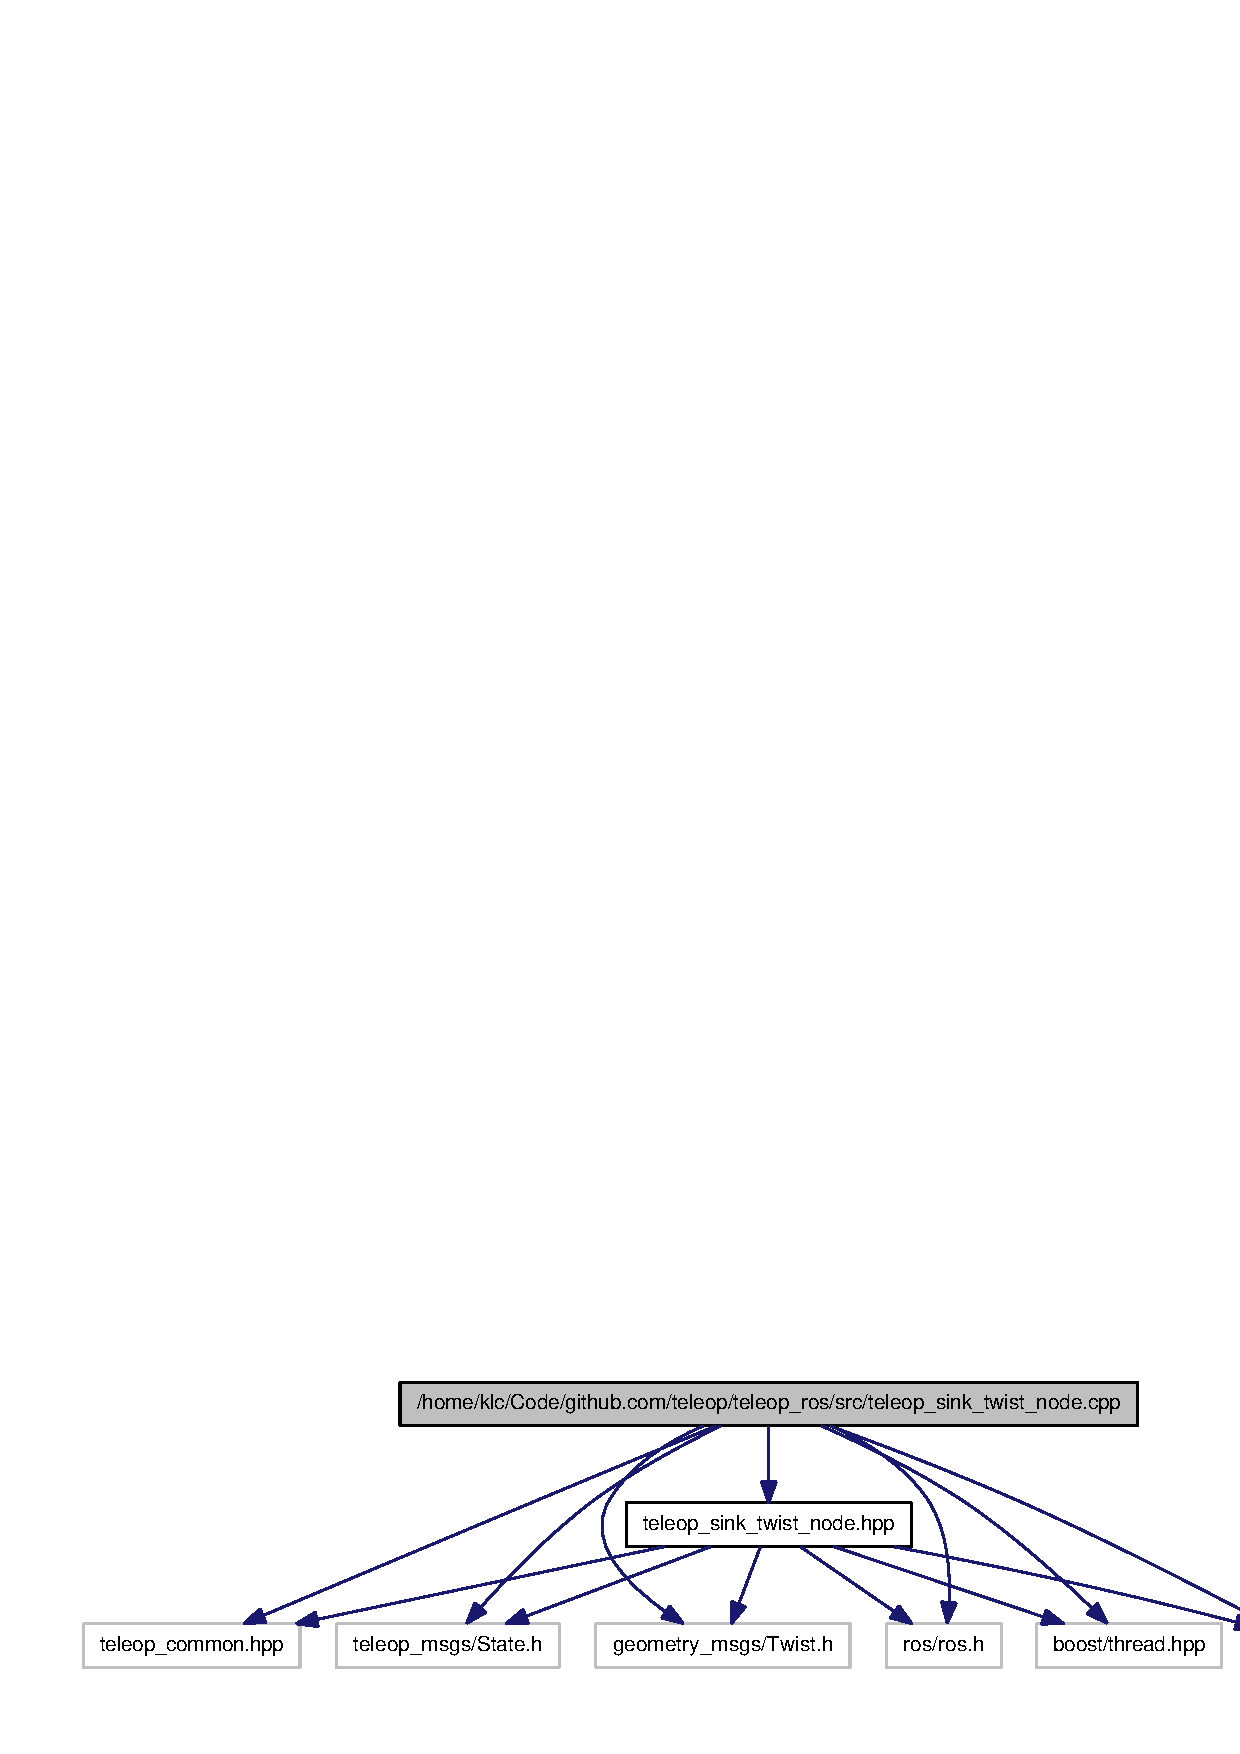
\includegraphics[width=400pt]{teleop__sink__twist__node_8cpp__incl}
\end{center}
\end{figure}
\subsection*{Functions}
\begin{DoxyCompactItemize}
\item 
int {\bf main} (int argc, char $\ast$$\ast$argv)
\end{DoxyCompactItemize}


\subsection{Function Documentation}
\index{teleop\_\-sink\_\-twist\_\-node.cpp@{teleop\_\-sink\_\-twist\_\-node.cpp}!main@{main}}
\index{main@{main}!teleop_sink_twist_node.cpp@{teleop\_\-sink\_\-twist\_\-node.cpp}}
\subsubsection[{main}]{\setlength{\rightskip}{0pt plus 5cm}int main (
\begin{DoxyParamCaption}
\item[{int}]{argc, }
\item[{char $\ast$$\ast$}]{argv}
\end{DoxyParamCaption}
)}\label{teleop__sink__twist__node_8cpp_a3c04138a5bfe5d72780bb7e82a18e627}


Definition at line 976 of file teleop\_\-sink\_\-twist\_\-node.cpp.


\section{teleop\_\-source\_\-node.cpp File Reference}
\label{teleop__source__node_8cpp}\index{teleop\_\-source\_\-node.cpp@{teleop\_\-source\_\-node.cpp}}
{\ttfamily \#include $<$teleop\_\-source\_\-node.hpp$>$}\par
{\ttfamily \#include $<$teleop\_\-common.hpp$>$}\par
{\ttfamily \#include $<$teleop\_\-source.hpp$>$}\par
{\ttfamily \#include $<$teleop\_\-source\_\-adapter.hpp$>$}\par
{\ttfamily \#include $<$teleop\_\-source\_\-keyboard.hpp$>$}\par
{\ttfamily \#include $<$teleop\_\-source\_\-joystick.hpp$>$}\par
{\ttfamily \#include $<$teleop\_\-msgs/State.h$>$}\par
{\ttfamily \#include $<$ros/ros.h$>$}\par
{\ttfamily \#include $<$boost/thread.hpp$>$}\par
{\ttfamily \#include $<$stdint.h$>$}\par
Include dependency graph for teleop\_\-source\_\-node.cpp:
\nopagebreak
\begin{figure}[H]
\begin{center}
\leavevmode
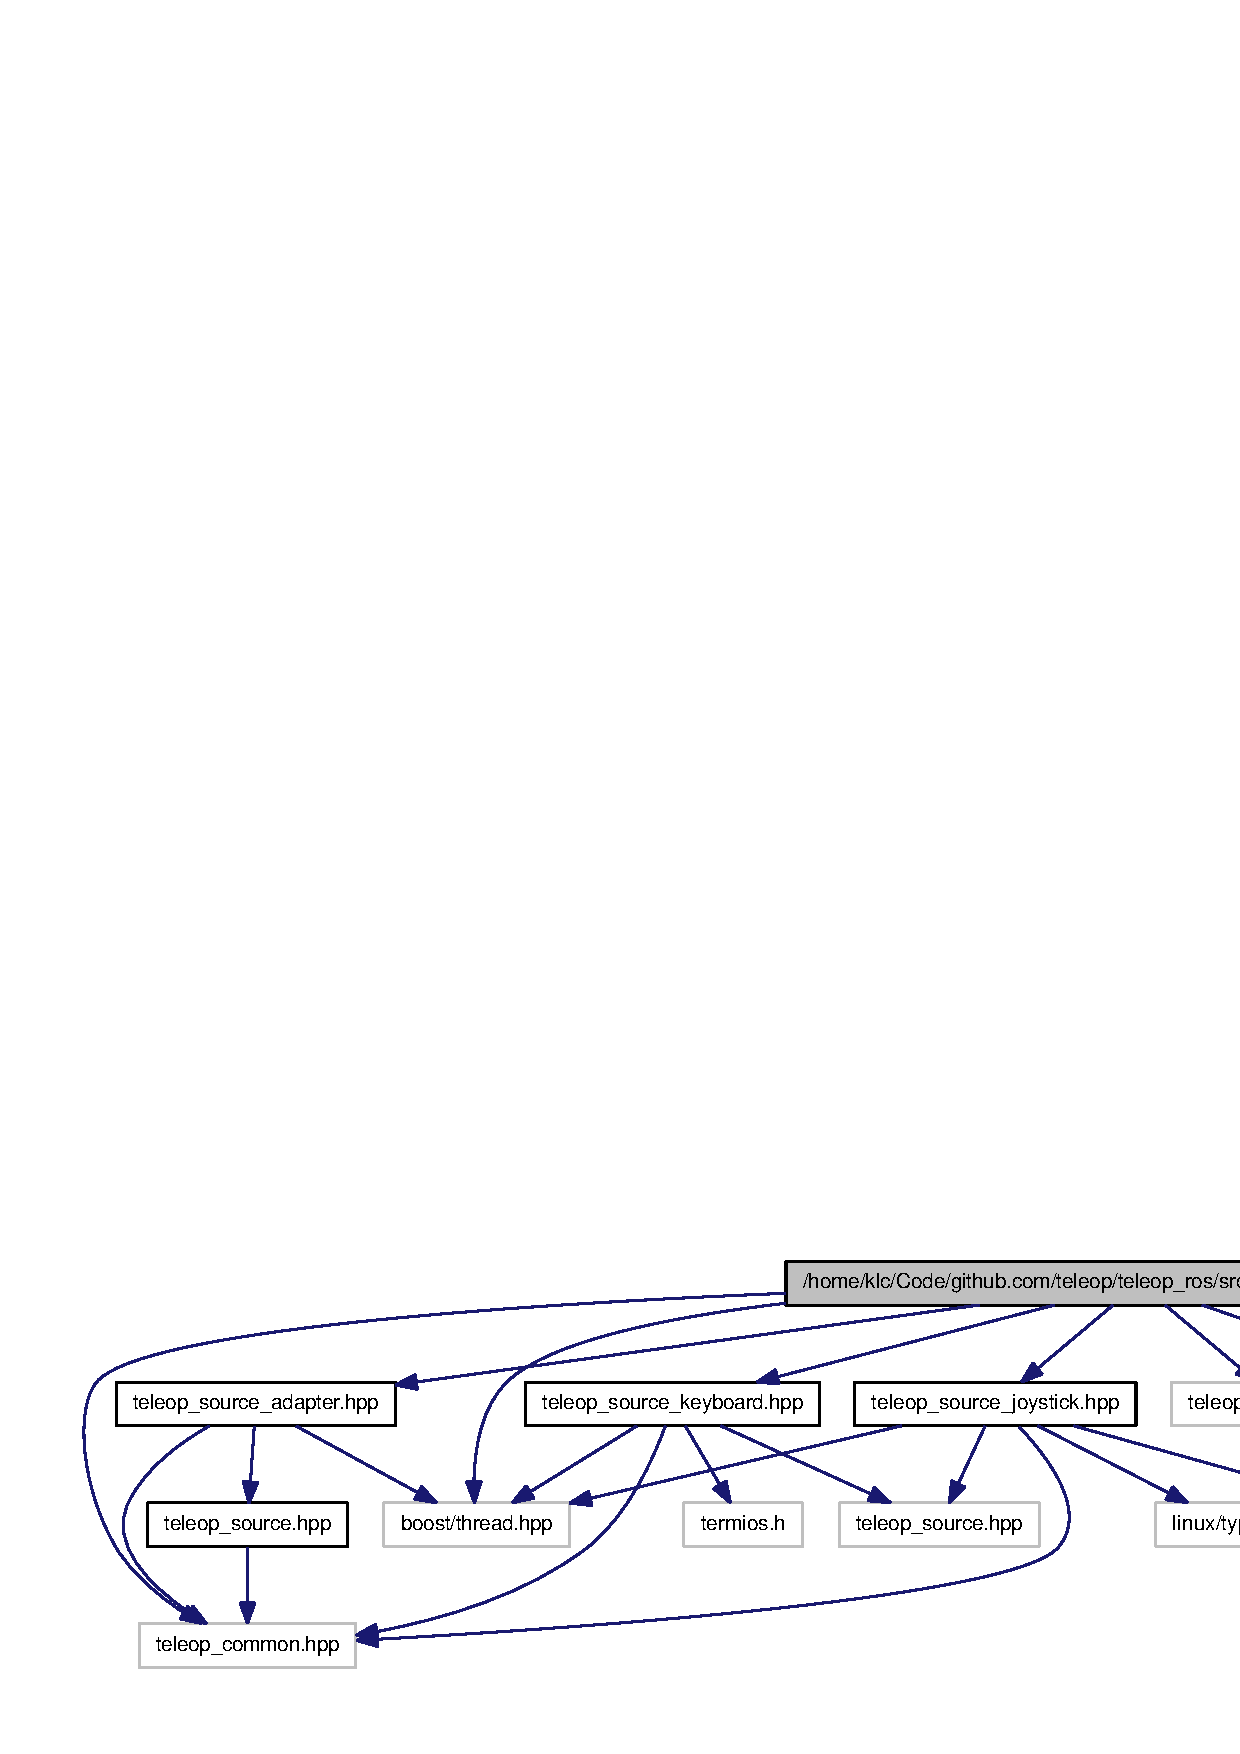
\includegraphics[width=400pt]{teleop__source__node_8cpp__incl}
\end{center}
\end{figure}
\subsection*{Namespaces}
\begin{DoxyCompactItemize}
\item 
namespace {\bf teleop}
\end{DoxyCompactItemize}

\printindex
\end{document}
